


\tikzset{every picture/.style={line width=0.75pt}} %set default line width to 0.75pt        

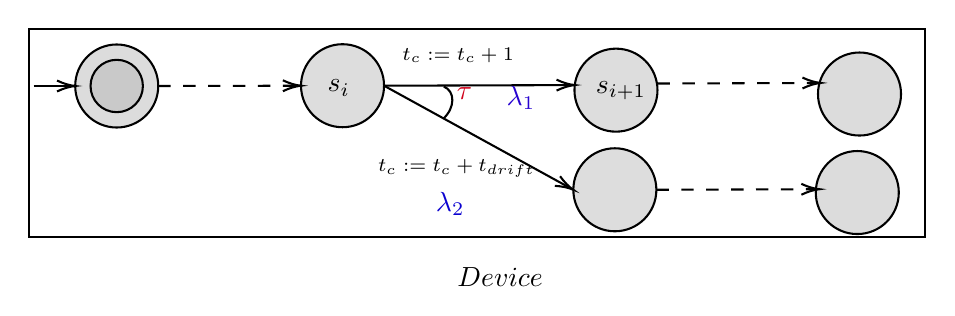
\begin{tikzpicture}[x=0.60pt,y=0.60pt,yscale=-1,xscale=1]
%uncomment if require: \path (0,300); %set diagram left start at 0, and has height of 300

%Shape: Circle [id:dp0800372807837828] 
\draw  [fill={rgb, 255:red, 155; green, 155; blue, 155 }  ,fill opacity=0.34 ] (193.33,42.5) .. controls (193.33,28.69) and (204.53,17.5) .. (218.33,17.5) .. controls (232.14,17.5) and (243.33,28.69) .. (243.33,42.5) .. controls (243.33,56.31) and (232.14,67.5) .. (218.33,67.5) .. controls (204.53,67.5) and (193.33,56.31) .. (193.33,42.5) -- cycle ;
%Shape: Circle [id:dp6517135602121005] 
\draw  [fill={rgb, 255:red, 155; green, 155; blue, 155 }  ,fill opacity=0.34 ] (358,45.17) .. controls (358,31.36) and (369.19,20.17) .. (383,20.17) .. controls (396.81,20.17) and (408,31.36) .. (408,45.17) .. controls (408,58.97) and (396.81,70.17) .. (383,70.17) .. controls (369.19,70.17) and (358,58.97) .. (358,45.17) -- cycle ;
%Shape: Circle [id:dp020288374699267364] 
\draw  [fill={rgb, 255:red, 155; green, 155; blue, 155 }  ,fill opacity=0.35 ] (504.67,47.5) .. controls (504.67,33.69) and (515.86,22.5) .. (529.67,22.5) .. controls (543.47,22.5) and (554.67,33.69) .. (554.67,47.5) .. controls (554.67,61.31) and (543.47,72.5) .. (529.67,72.5) .. controls (515.86,72.5) and (504.67,61.31) .. (504.67,47.5) -- cycle ;
%Shape: Circle [id:dp8120002198294831] 
\draw  [fill={rgb, 255:red, 155; green, 155; blue, 155 }  ,fill opacity=0.35 ] (57.33,42.67) .. controls (57.33,28.86) and (68.53,17.67) .. (82.33,17.67) .. controls (96.14,17.67) and (107.33,28.86) .. (107.33,42.67) .. controls (107.33,56.47) and (96.14,67.67) .. (82.33,67.67) .. controls (68.53,67.67) and (57.33,56.47) .. (57.33,42.67) -- cycle ;
%Straight Lines [id:da06780717013530502] 
\draw  [dash pattern={on 4.5pt off 4.5pt}]  (107.33,42.67) -- (191.33,42.5) ;
\draw [shift={(193.33,42.5)}, rotate = 179.89] [color={rgb, 255:red, 0; green, 0; blue, 0 }  ][line width=0.75]    (10.93,-3.29) .. controls (6.95,-1.4) and (3.31,-0.3) .. (0,0) .. controls (3.31,0.3) and (6.95,1.4) .. (10.93,3.29)   ;
%Straight Lines [id:da8484939119584262] 
\draw    (243.33,42.5) -- (356.15,42.12) ;
\draw [shift={(358.15,42.11)}, rotate = 179.81] [color={rgb, 255:red, 0; green, 0; blue, 0 }  ][line width=0.75]    (10.93,-3.29) .. controls (6.95,-1.4) and (3.31,-0.3) .. (0,0) .. controls (3.31,0.3) and (6.95,1.4) .. (10.93,3.29)   ;
%Straight Lines [id:da5499753499142862] 
\draw  [dash pattern={on 4.5pt off 4.5pt}]  (408,41.17) -- (504.25,40.84) ;
\draw [shift={(506.25,40.83)}, rotate = 179.81] [color={rgb, 255:red, 0; green, 0; blue, 0 }  ][line width=0.75]    (10.93,-3.29) .. controls (6.95,-1.4) and (3.31,-0.3) .. (0,0) .. controls (3.31,0.3) and (6.95,1.4) .. (10.93,3.29)   ;
%Straight Lines [id:da8750765790283018] 
\draw    (32.33,42.67) -- (55.33,42.67) ;
\draw [shift={(57.33,42.67)}, rotate = 180] [color={rgb, 255:red, 0; green, 0; blue, 0 }  ][line width=0.75]    (10.93,-3.29) .. controls (6.95,-1.4) and (3.31,-0.3) .. (0,0) .. controls (3.31,0.3) and (6.95,1.4) .. (10.93,3.29)   ;
%Shape: Circle [id:dp9577830715523987] 
\draw  [fill={rgb, 255:red, 155; green, 155; blue, 155 }  ,fill opacity=0.29 ] (66.56,42.67) .. controls (66.56,33.96) and (73.62,26.9) .. (82.33,26.9) .. controls (91.04,26.9) and (98.1,33.96) .. (98.1,42.67) .. controls (98.1,51.38) and (91.04,58.44) .. (82.33,58.44) .. controls (73.62,58.44) and (66.56,51.38) .. (66.56,42.67) -- cycle ;
%Shape: Rectangle [id:dp759633067613265] 
\draw   (29.33,8.17) -- (569.29,8.17) -- (569.29,133.8) -- (29.33,133.8) -- cycle ;
%Shape: Circle [id:dp5232490962749833] 
\draw  [fill={rgb, 255:red, 155; green, 155; blue, 155 }  ,fill opacity=0.34 ] (357.33,105.17) .. controls (357.33,91.36) and (368.53,80.17) .. (382.33,80.17) .. controls (396.14,80.17) and (407.33,91.36) .. (407.33,105.17) .. controls (407.33,118.97) and (396.14,130.17) .. (382.33,130.17) .. controls (368.53,130.17) and (357.33,118.97) .. (357.33,105.17) -- cycle ;
%Shape: Circle [id:dp6752098325857876] 
\draw  [fill={rgb, 255:red, 155; green, 155; blue, 155 }  ,fill opacity=0.35 ] (503.33,106.83) .. controls (503.33,93.03) and (514.53,81.83) .. (528.33,81.83) .. controls (542.14,81.83) and (553.33,93.03) .. (553.33,106.83) .. controls (553.33,120.64) and (542.14,131.83) .. (528.33,131.83) .. controls (514.53,131.83) and (503.33,120.64) .. (503.33,106.83) -- cycle ;
%Straight Lines [id:da7293836315789196] 
\draw  [dash pattern={on 4.5pt off 4.5pt}]  (407.33,105.17) -- (503.58,104.84) ;
\draw [shift={(505.58,104.83)}, rotate = 179.81] [color={rgb, 255:red, 0; green, 0; blue, 0 }  ][line width=0.75]    (10.93,-3.29) .. controls (6.95,-1.4) and (3.31,-0.3) .. (0,0) .. controls (3.31,0.3) and (6.95,1.4) .. (10.93,3.29)   ;
%Straight Lines [id:da5166679562063851] 
\draw    (243.33,42.5) -- (355.58,104.2) ;
\draw [shift={(357.33,105.17)}, rotate = 208.8] [color={rgb, 255:red, 0; green, 0; blue, 0 }  ][line width=0.75]    (10.93,-3.29) .. controls (6.95,-1.4) and (3.31,-0.3) .. (0,0) .. controls (3.31,0.3) and (6.95,1.4) .. (10.93,3.29)   ;
%Curve Lines [id:da46003188830589814] 
\draw    (279.33,43) .. controls (286.24,45.8) and (286.24,55.8) .. (278.91,62.47) ;


% Text Node
\draw (285.33,42) node [anchor=north west][inner sep=0.75pt]  [color={rgb, 255:red, 208; green, 2; blue, 27 }  ,opacity=1 ]  {$\tau $};
% Text Node
\draw (272.67,104.67) node [anchor=north west][inner sep=0.75pt]  [color={rgb, 255:red, 11; green, 2; blue, 208 }  ,opacity=1 ]  {$\boldsymbol{\lambda _{2}}$};
% Text Node
\draw (315.33,40.67) node [anchor=north west][inner sep=0.75pt]  [color={rgb, 255:red, 39; green, 2; blue, 208 }  ,opacity=1 ]  {$\boldsymbol{\lambda _{1}}$};
% Text Node
\draw (237.83,85.33) node [anchor=north west][inner sep=0.75pt]  [font=\scriptsize,color={rgb, 255:red, 0; green, 0; blue, 0 }  ,opacity=1 ]  {$\boldsymbol{t_{c} :=t_{c} +t_{drift}}$};
% Text Node
\draw (285.67,150) node [anchor=north west][inner sep=0.75pt]    {$Device\ $};
% Text Node
\draw (252.5,17.67) node [anchor=north west][inner sep=0.75pt]  [font=\scriptsize,color={rgb, 255:red, 0; green, 0; blue, 0 }  ,opacity=1 ]  {$\boldsymbol{t_{c} :=t_{c} +1}$};
% Text Node
\draw (369.03,38.17) node [anchor=north west][inner sep=0.75pt]    {$s_{i+1}$};
% Text Node
\draw (207.53,37.17) node [anchor=north west][inner sep=0.75pt]    {$s_{i}$};


\end{tikzpicture}
